\documentclass[a4paper]{article} 
\input{head}
\usepackage[T1]{fontenc}
\usepackage[utf8]{vietnam}
\usepackage{graphicx}
\usepackage{pgfplots}
\pgfplotsset{width=10cm,compat=1.9}
\usepackage{animate}
\usepgfplotslibrary{external}
\tikzexternalize
\usepackage{amsmath}
\setlength{\parskip}{0.5em}
\begin{document}

%-------------------------------
%	TITLE SECTION
%-------------------------------

\fancyhead[C]{}
\hrule \medskip % Upper rule
\begin{minipage}{0.295\textwidth} 
\raggedright
\footnotesize
VŨ QUANG HẢI \hfill\\
16003499 - K61A2\hfill\\
\href{mailto: vuquanghai_t61@hus.edu.vn}{vuquanghai\_t61@hus.edu.vn}
\end{minipage}
\begin{minipage}{0.4\textwidth}
\centering 
\large 
Phương trình truyền sóng một chiều \\ 
\normalsize 
Phương trình đạo hàm riêng, MAT 2306 1 \\ 
\end{minipage}
\begin{minipage}{0.295\textwidth} 
\raggedleft
\today\hfill\\
\end{minipage}
\medskip\hrule 
\bigskip

%-------------------------------
%	CONTENTS
%-------------------------------

\section{Mở đầu}
Bài tiểu luận này sẽ nói về \emph{phương trình truyền sóng một chiều}. Để minh hoạ đơn giản nhất về dạng phương trình truyền sóng này, ta có thể liên tưởng đến việc lan truyền một gợn sóng trên một sợi dây thừng hay hình dáng dao động của dây đàn guitar khi đang được gẩy. Mục đích của phương trình truyền sóng là khảo sát sự lan truyền của sóng.

\section{Bài toán Cauchy cho phương trình truyền sóng thuần nhất}
\subsection{Mô tả phương trình truyền sóng dạng thuần nhất}

Một phương trình truyền sóng thuần nhất là một phương trình đạo hàm riêng cấp hai có dạng:
\begin{equation*}
\begin{aligned}[t]
u_{tt} - c^2u_{xx} = 0
\end{aligned}
\qquad
\begin{aligned}[t]
t > 0, x \in \mathbb{R}, c \in \mathbb{R}^+
\end{aligned}
\qquad
\begin{aligned}[t]
(1)
\end{aligned}
\end{equation*}

Trong công thức trên, ta có hằng số $c$ là \emph{tốc độ lan truyền sóng}. Ý nghĩa của hằng số này sẽ được mô tả ở dưới.

\subsection{Nghiệm tổng quát của dạng thuần nhất}

Vì phương trình truyền sóng cũng là một phương trình đạo hàm riêng cấp hai, ta có thể dùng phương pháp đặc trưng để giải phương trình này. Trước hết ta sẽ đưa phương trình về dạng chính tắc. Từ phương trình trên, ta có phương trình đặc trưng cho phương trình đạo hàm riêng cấp hai như sau:

\begin{equation*}
(dx)^2 - c^2(dt)^2 = 0
\end{equation*}
Dễ thấy $\Delta > 0$, tức phương trình trên có dạng hyperbolic. Từ đó ta có hai công thức nghiệm nghiệm của phương trình đặc trưng trên như sau:
\begin{equation*}
\begin{aligned}[t]
x - ct = C_1
\end{aligned}
\qquad
\begin{aligned}[t]
x + ct = C_2
\end{aligned}
\end{equation*}

Tại bước này, ta đổi biến phương trình đạo hàm riêng trên:

\begin{equation*}
\begin{aligned}[t]
\xi &= x - ct
\end{aligned}
\qquad
\begin{aligned}[t]
\eta &= x + ct
\end{aligned}
\end{equation*}

Từ đó thu được phương trình chính tắc có dạng $v(\xi(x, t), \eta(x, t))$. Để xác định dạng chính tắc này ta lập bảng đạo hàm riêng:

\begin{center}
\begin{tabular}{|c|c|c|c|c|c|c|}
\hline
       &          & $v_\xi$ & $v_\eta$ & $v_{\xi\xi}$ & $v_{\xi\eta}$ & $v_{\eta\eta}$ \\
\hline
$0$    & $u_x$    & $1$     & $1$      & $0$          & $0$           & $0$            \\
$0$    & $u_t$    & $c$     & $-c$     & $0$          & $0$           & $0$            \\
$-c^2$ & $u_{xx}$ & $0$     & $0$      & $1$          & $2$           & $1$            \\
$0$    & $u_{xt}$ & $0$     & $0$      & $1$          & $0$           & $-c^2$         \\
$1$    & $u_{tt}$ & $0$     & $0$      & $c^2$        & $-2c^2$       & $c^2$          \\
\hline
$0$    & $0$      & $0$     & $0$      & $0$          & $-4c^2$       & $0$            \\
\hline
\end{tabular}
\end{center}

Từ đây suy ra phương trình chính tắc của bài toán là $-4c^2v_{\xi\eta} = 0$. Ở trên ta đã biết được phương trình này thuộc đạng hyperbolic nên ta có nghiệm tổng quát của phương trình như sau:

\begin{equation*}
u(x, y) = F(x - ct) + G(x + ct)
\end{equation*}

Qua kết quả trên, ta có thể thấy quá trình truyền sóng là sự kết hợp của hai hàm là $F$ và $G$. Hàm $F(x - ct)$ và $G(x + ct)$ thực chất là chính là hàm số $F(x)$ và $G(x)$ đã tịnh tiến về hai chiều khác nhau. Hàm $F(x - ct)$ sẽ tịnh tiến về phía trái, gọi là \emph{sóng lùi}, hàm $G(x + ct)$ tịnh tiến về phía ngược lại, gọi là \emph{sóng tiến}.

\subsection{Giải bài toán Cauchy}
Từ phương trình truyền sóng thuần nhất đã nêu ở trên, ta thêm hai điều kiện ban đầu như sau để được bài toán Cauchy:
\begin{equation*}
\begin{aligned}[t]
u_{tt} - c^2u_{xx} = 0
\end{aligned}
\qquad
\begin{aligned}[t]
c \in \mathbb{R}^+
\end{aligned}
\end{equation*}
\begin{equation*}
\begin{aligned}[t]
u(x, 0) &= f(x)
\end{aligned}
\qquad
\begin{aligned}[t]
u_t(x, 0) &= g(x)
\end{aligned}
\qquad
\begin{aligned}[t]
x \in \mathbb{R}
\end{aligned}
\qquad
\begin{aligned}[t]
(2)
\end{aligned}
\end{equation*}

Về ý tưởng, $u(x, 0)$ là hình dạng hay biên độ sóng, $u_t(x, 0)$ chính là vận tốc của sóng, đều tại thời gian bắt đầu truyền sóng. Hướng để giải quyết của bài toán là tìm hàm $F$ và $G$ trong phương trình nghiệm tổng quát sao cho hai hàm đó thoả mãn điều khiện ban đầu. Cho $t = 0$ vào nghiệm tổng quát, ta có điều kiện ban đầu đầu như sau:

\begin{equation*}
\begin{aligned}[t]
u(x,0) = F(x) + G(x) = f(x)
\end{aligned}
\qquad
\begin{aligned}[t]
(*)
\end{aligned}
\end{equation*}

Đạo hàm theo $t$ công thức nghiệm tổng quát của phương trình truyền sóng, sau đó cho $t = 0$, ta sẽ có điều kiện ban đầu thứ hai:
\begin{equation*}
u_t(x,0) = cF'(x) + cG'(x) = g(x)
\end{equation*}

Sau đó tích phân hai vế của phương trình này trong đoạn $[0, x]$, ta được:

\begin{equation*}
\begin{aligned}[t]
F(x) - G(x) = \frac{1}{c} \int_{0}^{x} g(s) \,ds + C
\end{aligned}
\qquad
\begin{aligned}[t]
(**)
\end{aligned}
\end{equation*}

Từ $(*)$ và $(**)$, ta giải hệ hai phương trình trên và thu được:

\begin{equation*}
F(x) = \frac{f(x)}{2} + \frac{1}{2c} \int_{0}^{x} g(s) \,ds + \frac{C}{2}
\end{equation*}
\begin{equation*}
G(x) = \frac{f(x)}{2}  - \frac{1}{2c} \int_{0}^{x} g(s) \,ds - \frac{C}{2}
\end{equation*}

Lắp $F(x)$ và $G(x)$ và công thức nghiệm ban đầu, ta có được nghiệm tổng quát của bài toán Cauchy:

\begin{equation*}
u(x, t) = \frac{f(x + ct) + f(x - ct)}{2} + \frac{1}{2c} \int_{x - ct}^{x + ct} g(s) \, ds
\end{equation*}

Phương trình này còn có tên gọi khác là \emph{công thức d'Alembert}. Từ công thức này ta dễ dàng tìm ra biên độ của sóng tại mọi điểm trong mọi thời gian.

\subsubsection{Tính chất của nghiệm phương trình truyền sóng}

Ở trên, ta đã tìm công thức d'Alembert cho phương trình truyền sóng. Nếu các điều kiện ban đầu của $u(x, 0)$ và $u_t(x, 0)$ đủ tốt, cụ thể là $f \in C^2(\mathbb{R})$, $g \in C^1(\mathbb{R})$ với $t \geq 0$ thì nghiệm $u(x, t)$ sẽ khả vi đến cấp $2$ và và nó thoả mãn phương trình truyền sóng và các điều kiện ban đầu theo nghĩa thông thường. Lúc này, hiển nhiên $u(x, t)$ cũng sẽ kế thừa được tất cả các tính chất của điều kiện ban đầu (khả vi tại mọi điểm), ta gọi là \emph{nghiệm cổ điển}. Nhưng nếu các điều kiện ban đầu không thoả mãn tính chất khả vi, liệu có thể nhanh chóng kết luận rằng nghiệm thu được không phải là nghiệm cổ điển?

Để lấy ví dụ, giả sử ta có phép toán tổng ($+$) và hai số thực $a$ và $b$ trong trường $\mathbb{R}$ và $c$ là tổng của hai số trên. Tổng $c$ được gọi là tốt khi $c$ là số hữu tỉ và xấu khi là số vô tỉ. Trong môn giải tích hàm, ta dễ dàng chứng minh được rằng nếu $a$ và $b$ là hai số hữu tỉ, thì $c$ cũng là một số hữu tỉ (ánh xạ của hai tập hữu hạn vào tập đích cũng phải là tập hữu hạn). Nhưng nếu $a$ và $b$ là số vô tỉ, thì không chắc chắn rằng $c$ cũng là vô tỉ bằng phép chứng mình phản chứng: tổng $\pi + (-\pi) = 0$ là số hữu tỉ. Tương tự, với nghiệm của phương trình truyền sóng, tổng của hai hàm không liên tục chưa chắc đã không sinh ra nghiệm cổ điển. Ta phải xét các tất cả tính khả vi của nghiệm, rồi sau đó mới đưa ra được kết luận đó có phải nghiệm cổ điển hay không.

\subsection{Sử dụng đồ thị giải nghiệm bài toán Cauchy}

Phương pháp đồ thị là một cách trực quan và thú vị để thấy được hình dạng và tính chất của sóng. Trước khi đi vào phương pháp này, ta cần phải làm rõ một vài lý thuyết dưới đây.

\subsubsection{Đường đặc trưng của phương trình truyền sóng}

Từ nghiệm của bài toán Cauchy, ta chọn lấy một điểm $(x_0, t_0)$, lắp vào công thức d'Alembert để được một nghiệm riêng như sau:

\begin{equation*}
u(x_0, t_0) = \frac{f(x_0 + ct_0) + f(x_0 - ct_0)}{2} + \frac{1}{2c} \int_{x_0 - ct_0}^{x_0+ct_0} g(s) \,ds
\end{equation*}

Trên mặt phẳng $(x, t)$, ta lấy hai đường thẳng đi qua điểm $(x_0, t_0)$ như sau:

\begin{equation*}
\begin{aligned}[t]
x - ct = x_0 - ct_0
\end{aligned}
\qquad
\begin{aligned}[t]
x + ct = x_0 + ct_0
\end{aligned}
\end{equation*}

Hai đường thẳng này giao trục $x$ tại $(x_0 - ct_0, 0)$, $(x_0 + ct_0, 0)$ và giao nhau tại điểm $(x_0, t_0)$. Tam giác hình thành bởi hai đường thẳng và trục $x$ được gọi là \emph{tam giác đặc trưng}.

\begin{center} 
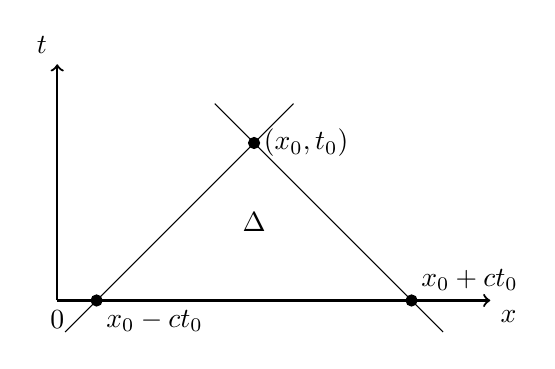
\begin{tikzpicture}
% \draw[step=1cm,gray,very thin] (-0.5,-0.5) grid (6.5,3.5);

\draw[thick,->] (0.5,0) -- (6,0) node[anchor=north west] {$x$};
\draw[thick,->] (0.5,0) -- (0.5,3) node[anchor=south east] {$t$};
\draw (0.5 cm, 0pt) node[anchor=north] {$0$};

\draw (0.6,-0.4) -- (3.5,2.5);
\draw (5.4,-0.4) -- (2.5,2.5);
\filldraw[black] (3,2) circle (2pt) node[anchor=west] {$(x_0, t_0)$};
\filldraw[black] (1,0) circle (2pt) node[anchor=north west] {$x_0 - ct_0$};
\filldraw[black] (5,0) circle (2pt) node[anchor=south west] {$x_0 + ct_0$};

\node[] at (3, 1) {$\Delta$};
\end{tikzpicture}
\end{center}

Qua hình vẽ trên, ta có thể mô tả tính chất hình học của công thức d'Alembert như sau:

\emph{Nghiệm riêng của một phương trình truyền sóng tại điểm $(x_0, t_0)$ là tổng của hai yếu tố sau:
\begin{itemize}
\item Trung bình cộng của biên độ sóng ban đầu tại hai điểm $(x_0 - ct_0,0)$ và $(x_0 + ct_0,0)$
\item Diện tích hàm vận tốc truyền sóng ban đầu tại hai điểm trong đoạn $[x_0 - ct, x_0 + ct_0]$
\end{itemize}}

Nhận xét: giá trị của $(x_0, t_0)$ hoàn toàn chỉ phụ thuộc vào điều kiện ban đầu trong đoạn $[x_0 - ct, x_0 + ct_0]$. Ta gọi đoạn này là \emph{miền phụ thuộc}. Nếu có các hàm điều kiện ban đầu có bị thay đổi, miễn là trong miền phụ thuộc hàm vẫn giữ nguyên, thì giá trị của $(x_0, t_0)$ sẽ không bị thay đổi theo.

Ngược lại, ta sẽ có một nhận xét rộng hơn rằng, đường đặc trưng có đại diện được tập hợp các điểm $(x_0, t_0)$ đại diện cho sự ảnh hưởng của các điều kiện ban đầu trong một đoạn $[a, b]$ (tất nhiên với điều kiện $[a, b] \cap [x_0 - ct, x_0 + ct_0] \neq \emptyset$)? Câu trả lời là có, đó là tập hợp các điểm $(x_0, t_0)$ thoả mãn điều kiện:

\begin{equation*}
\begin{aligned}[t]
x - ct \leq b
\end{aligned}
\qquad
\begin{aligned}[t]
và
\end{aligned}
\qquad
\begin{aligned}[t]
x + ct \geq a
\end{aligned}
\end{equation*}

Vùng thoả mãn điều kiện trên được gọi là \emph{vùng ảnh hưởng}. Để minh hoạ, thì đó là vùng màu đỏ ở hình vẽ:

\begin{center} 
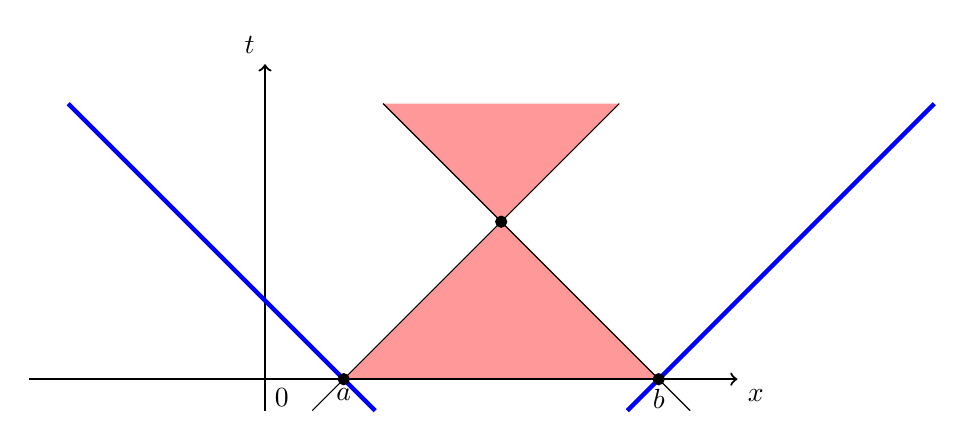
\begin{tikzpicture}
\fill[red!40!white] (1,0) -- (4.5,3.5) -- (1.5,3.5) -- (5, 0);

\draw[thick,->] (-3,0) -- (6,0) node[anchor=north west] {$x$};
\draw[thick,->] (0,-0.4) -- (0,4) node[anchor=south east] {$t$};
\draw (0 cm, 0pt) node[anchor = north west] {$0$};

\draw (0.6,-0.4) -- (4.5,3.5);
\draw (5.4,-0.4) -- (1.5,3.5);
\draw[ultra thick, blue] (1.4,-0.4) -- (-2.5,3.5);
\draw[ultra thick, blue] (4.6,-0.4) -- (8.5,3.5);

\filldraw[black] (3,2) circle (2pt) node[anchor=west] {};
\filldraw[black] (1,0) circle (2pt) node[anchor=north] {$a$};
\filldraw[black] (5,0) circle (2pt) node[anchor=north] {$b$};
\end{tikzpicture}
\end{center}

Giả sử hàm $f$ và $g$ chỉ khác $0$ trong đoạn $[a, b]$, công thức d'Alembert chỉ có ý nghĩa trong mặt phẳng được giới hạn bởi miền $x - ct \leq a$ và $x + ct \geq b$ (chính là hình nón rộng giới hạn bời đường màu xanh chứa vùng ảnh hưởng của hình vẽ trên).

Để ví dụ, ta có bài toán Cauchy đơn giản như sau:

\begin{equation*}
\begin{aligned}[t]
u_{tt} - c^2u_{xx} = 0
\end{aligned}
\qquad
\begin{aligned}[t]
x \in \mathbb{R}, t \leq 0
\end{aligned}
\end{equation*}

\begin{equation*}
u(x, 0) = f(x) = 
\begin{cases}
1 & |x| \leq a \\
0 & |x| \geq a 
\end{cases}
\end{equation*}

\begin{equation*}
u-t(x, 0) = g(x) = 0
\end{equation*}

Sử dụng công thức d'Alembert, ta có tổng của sóng tiến và sóng lùi như sau:

\begin{equation*}
u(x, t) = \frac{f(x + ct) + f(x - ct)}{2}
\end{equation*}

Ta minh hoạ như hình dưới đây, ta chỉ kẻ các đường đặc trưng đặc biệt, màu xanh lá chính là \emph{vùng ảnh hưởng}:

\begin{center} 
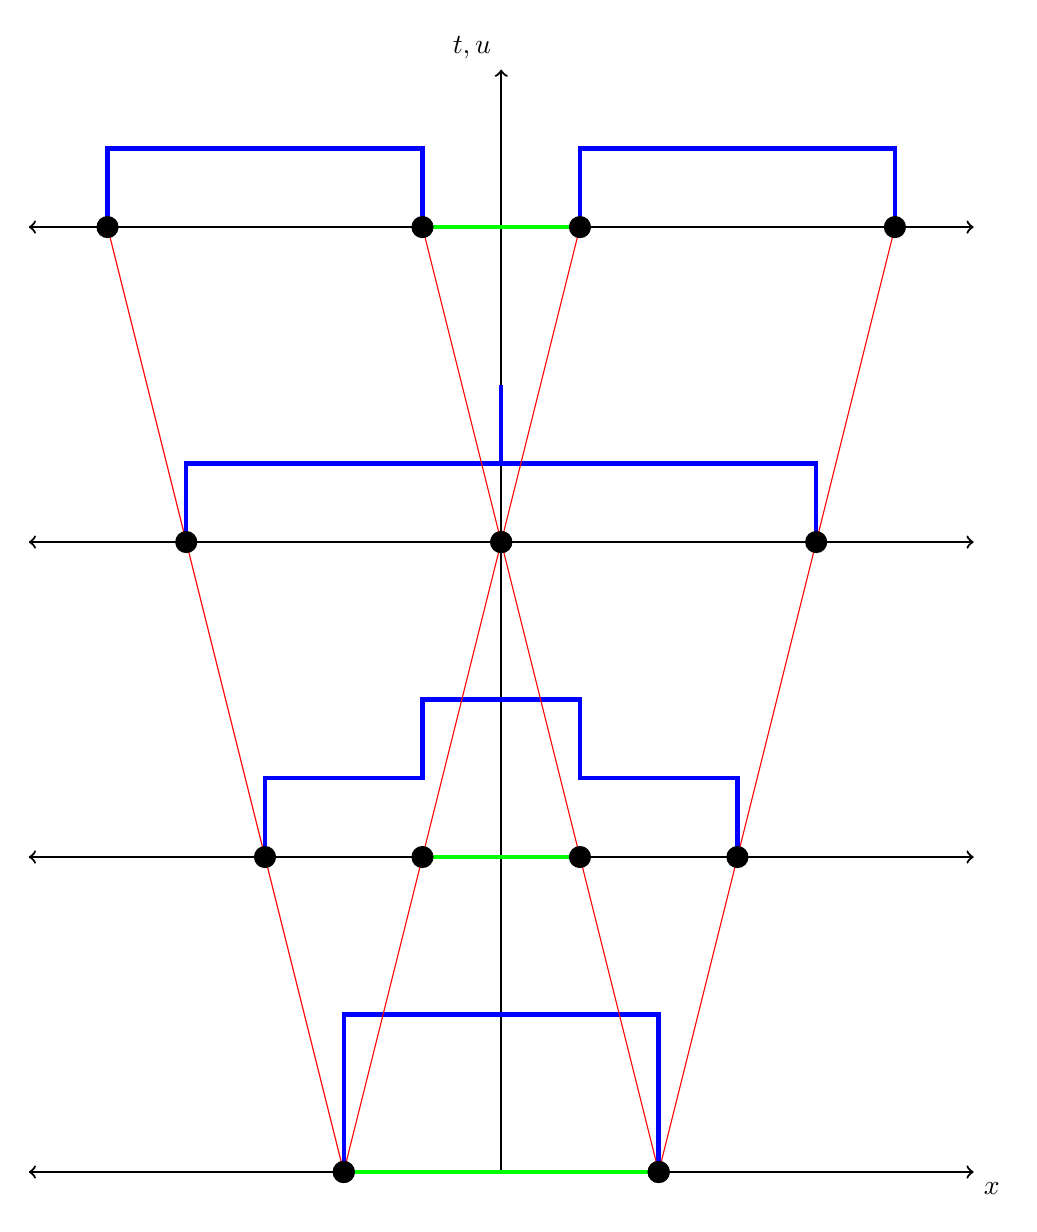
\begin{tikzpicture}

\draw[thick,<->] (-6,0) -- (6,0) node[anchor=north west] {$x$};
\draw[thick,<->] (-6,4) -- (6,4) node[anchor=north west] {};
\draw[thick,<->] (-6,8) -- (6,8) node[anchor=north west] {};
\draw[thick,<->] (-6,12) -- (6,12) node[anchor=north west] {};
\draw[thick,->] (0,0) -- (0,14) node[anchor=south east] {$t,u$};

\draw[ultra thick, blue] (-2,0) -- (-2, 2) -- (2,2) -- (2, 0);
\draw[ultra thick, blue] (-3,4) -- (-3, 5) -- (-1,5) -- (-1, 6) -- (1,6) -- (1,5) -- (3,5) -- (3,4);
\draw[ultra thick, blue] (-4,8) -- (-4, 9) -- (4, 9) -- (4, 8);
\draw[ultra thick, blue] (0,9) -- (0,10);
\draw[ultra thick, blue] (-5,12) -- (-5, 13) -- (-1, 13) -- (-1, 12);
\draw[ultra thick, blue] (5,12) -- (5, 13) -- (1, 13) -- (1, 12);

\draw[thin, red] (2,0) -- (5,12);
\draw[thin, red] (2,0) -- (-1, 12);
\draw[thin, red] (-2,0) -- (-5,12);
\draw[thin, red] (-2,0) -- (1,12);

\foreach \a in {0, 1, 2, 3} {
    \draw[ultra thick, green] (-2+\a,4*\a) -- (2-\a,4*\a);
    \fill[black] (-2+\a, 4*\a) circle (4pt);
    \fill[black] (-2-\a, 4*\a) circle (4pt);
    \fill[black] (2+\a, 4*\a) circle (4pt);
    \fill[black] (2-\a, 4*\a) circle (4pt);
}

\end{tikzpicture}
\end{center}

Để thêm phong phú, ta sẽ lấy một ví dụ khác mà sóng bị ảnh hưởng bởi vận tốc truyền sóng ban đầu. Dưới đây là một bài toán Cauchy như vậy:

\begin{equation*}
\begin{aligned}[t]
u_{tt} - u_{xx} = 0
\end{aligned}
\qquad
\begin{aligned}[t]
x \in \mathbb{R}, t \leq 0
\end{aligned}
\end{equation*}

\begin{equation*}
u(x, 0) = f(x) = 
\begin{cases}
8x - x^2 & 0 < x < 4  \\
0 & x > 0, x < 4
\end{cases}
\end{equation*}

\begin{equation*}
u_t(x, 0) = F(x) = 
\begin{cases}
16 & 0 < x < 4  \\
0 & x > 0, x < 4
\end{cases}
\end{equation*}

Do hàm này là hàm gián đoạn và không trơn, việc thay trực tiếp $f$ và $g$ vào công thức d'Alembert để tính nghiệm khá phức tạp, vậy nên ta sẽ sử dụng cách khác đơn giản hơn: Tính tổng sóng tiến và sóng lùi. Đã có nghiệm tổng quát dạng hyperbolic của phương trình truyền sóng đã chứng minh ở mục 2.2 là $u(x, y) = F(x - ct) + G(x + ct)$, ta sẽ tìm đi tìm công thức sóng tiến và sóng lùi như mục 2.3:

\begin{equation*}
F(x) = \frac{f(x)}{2}  + \frac{1}{2c} \int_{x}^{0} g(s) \,ds = 
\begin{cases}
0 & x < 0 \\
-4x-x^2 & 0 < x < 4 \\
-32 & x > 4
\end{cases}
\end{equation*}
\begin{equation*}
G(x) = \frac{f(x)}{2} - \frac{1}{2c} \int_{0}^{x} g(s) \,ds = 
\begin{cases}
0 & x < 0 \\
12x-x^2 & 0 < x < 4 \\
32 & x > 4
\end{cases}
\end{equation*}

Lắp $F$ và $G$ vào nghiệm của phương trình truyền sóng, ta có công thức nghiệm cụ thể như sau:
\begin{equation*}
    u(x,t) = \frac{f(x-t)}{2}  + \frac{1}{2c} \int_{x-t}^{0} g(s) \, ds + \frac{f(x+t)}{2} - \frac{1}{2c} \int_{0}^{x+t} g(s) \,ds
\end{equation*}

Dù thu được nghiệm cụ thể, nhưng để dễ tính ta vẫn sẽ tính tổng của $F(x - t) + G(x + t)$. Dưới đây là minh hoạ phương trình truyền sóng (truy cập đường dẫn sau \href{https://imgur.com/Kkt0MeT}{đường dẫn này} nếu hình minh hoạ dưới đây không chuyển động):

\begin{frame}{}
  \animategraphics[loop,controls,width=\linewidth]{30}{img/}{1}{180}
\end{frame}

\subsection{Bài toán Cauchy với điều kiện biên Dirichlet}

Như trong bài toán Cauchy cổ điển, sợi dây được coi như dài vô tận ở cả hai đầu. Nhưng trong thực tế, điều này rất khó có thể xảy ra, trừ khi ta khảo sát các sóng có bước sóng nhỏ trong một phạm vi hẹp. Thường sẽ có một điều kiện biên nào đó để giới hạn rung động của sợi dây truyền sóng, ví dụ như sợi dây đàn guitar, bị cố định tại phím đàn hoặc khoá đàn và ngựa đàn. Điều kiện biên như vậy gọi là \emph{điều kiện biên Dirichlet}. Dưới đây là dạng chung của bài toán Cauchy có điều kiện biên Dirichlet:

\begin{equation*}
\begin{aligned}[t]
u_{tt} - c^2u_{xx} = 0
\end{aligned}
\qquad
\begin{aligned}[t]
t > 0, 0 < x < l, c > 0
\end{aligned}
\end{equation*}

\begin{equation*}
\begin{aligned}[t]
u(x, 0) &= f(x)
\end{aligned}
\qquad
\begin{aligned}[t]
u_t(x, 0) &= g(x)
\end{aligned}
\qquad
\begin{aligned}[t]
x \in \mathbb{R}
\end{aligned}
\end{equation*}

\begin{equation*}
u(0, t) = u(l, t) = 0
\end{equation*}

Do điều kiện biên gắn với nghiệm đầu ra nên ta không thể dùng phương pháp đặc trưng để giải phương trình được nữa. Ta sẽ sử dụng một phương pháp tìm nghiệm từ dưới lên - phương pháp tách biến

Đầu tiên, giả sử nghiệm $u(x, t)$ có dạng tách biến như sau:

\begin{equation*}
    u(x, t) = X(x)T(t)
\end{equation*}

Đạo hàm nghiệm trên để lấy $u_{xx}$, $u_{tt}$, phương trình truyền sóng ban đầu ở trên trở thành:

\begin{equation*}
    X(x)T''(t) = c^2X''(x)T(t)
\end{equation*}

Chia cả hai vế cho $-c^2X(x)T(t)$, ta có:

\begin{equation*}
    -\frac{X''(x)}{X(x)} = -\frac{T''(t)}{c^2T(t)} = \lambda
\end{equation*}

Dễ thấy $\lambda$ là một hằng số và luôn dương (do điều kiện biên), đặt $\lambda = \beta^2$ với $\beta > 0$. Từ dữ kiện này viết được hai phương trình vi phân sau:

\begin{equation*}
\begin{aligned}[t]
T''(t) + c^2\beta^2T(t) = 0
\end{aligned}
\qquad
\begin{aligned}[t]
X''(x) + \beta^2X(x) = 0
\end{aligned}
\end{equation*}

Nghiệm của hai phương trình vi phân này là:

\begin{equation*}
\begin{aligned}[t]
T(t) = Acos\beta ct + Bsin\beta ct
\end{aligned}
\qquad
\begin{aligned}[t]
X(x) = Ccos\beta x + Dsin\beta x
\end{aligned}
\end{equation*}

Với $A$, $B$, $C$ và $D$ là các hằng số nào đó. Từ điều kiện biên, ta thay vào nghiệm tách biến như sau:

\begin{equation*}
X(0)T(t) = X(l)T(t) = 0
\end{equation*}

Ta bỏ qua trường hợp $T(t) \equiv 0$ do trường hợp này sẽ sinh ra nghiệm $u(x, t) = 0$ tầm thường. Ta sẽ xét trường hợp còn lại: $X(0) = X(l) = 0$. Thay nghiệm $X(x)$ tìm được ở trên vào phương trình này, ta có:

\begin{equation*}
\begin{aligned}[t]
X(0) = C = 0
\end{aligned}
\qquad
\begin{aligned}[t]
X(l) = Dsin\beta l = 0
\end{aligned}
\end{equation*}

Ta cũng sẽ bỏ qa trường hợp $D = 0$ vì cũng sẽ tìm nghiệm $u(x, t) = 0$ tầm thường. Như vậy chỉ còn trường hợp:

\begin{equation*}
\begin{aligned}[t]
sin\beta l = 0
\end{aligned}
\qquad
\begin{aligned}[t]
\Rightarrow
\end{aligned}
\qquad
\begin{aligned}[t]
\beta_n = \frac{n\pi}{l}
\end{aligned}
\qquad
\begin{aligned}[t]
n \in \mathbb{N}^*
\end{aligned}
\end{equation*}

Thay $\beta$ tìm được vào trên vào nghiệm tách biến $X(x)$, ta thu được:
\begin{equation*}
\begin{aligned}[t]
X_n(x) = sin\frac{n\pi}{l}
\end{aligned}
\qquad
\begin{aligned}[t]
n \in \mathbb{N}^*
\end{aligned}
\end{equation*}

với mỗi $n \in \mathbb{N}^*$, ta luôn tìm được một nghiệm tách biến tương ứng:

\begin{equation*}
    u_n(x,t) = (A_ncos\frac{n\pi}{l}ct + B_nsin\frac{n\pi}{l}ct)sin\frac{n\pi}{l}x
\end{equation*}

Do tổng của các nghiệm riêng cũng là một nghiệm của phương trình truyền sóng, ta sẽ có tổng hữu hạn sau là nghiệm tổng quát của phương trình:

\begin{equation*}
    u_n(x,t) = \sum_{n}^{}(A_ncos\frac{n\pi}{l}ct + B_nsin\frac{n\pi}{l}ct)sin\frac{n\pi}{l}x
\end{equation*}

Từ điều kiện ban đầu, ta sẽ có hệ phương trình sau để giải tìm lấy nghiệm chính xác của phương trình truyền sóng:

\begin{equation*}
u(x, 0) = f(x) \sum_{n}^{}sin\frac{n\pi}{l}x    
\end{equation*}
\begin{equation*}
u_t(x, 0) = g(x) \sum_{n}^{}\frac{n\pi c}{l}sin\frac{n\pi}{l}x    
\end{equation*}

%------------------------------------------------

\section{Bài toán Cauchy cho phương trình truyền sóng không thuần nhất}
\subsection{Mô tả bài toán}

Giả sử ta có bài toán Cauchy như sau:

\begin{equation*}
\begin{aligned}[t]
u_{tt} - c^2u_{xx} = F(x,t)
\end{aligned}
\qquad
\begin{aligned}[t]
t > 0, x \in \mathbb{R}, c \in \mathbb{R}^+
\end{aligned}
\end{equation*}

\begin{equation*}
\begin{aligned}[t]
u(x,0) = f(x)
\end{aligned}
\qquad
\begin{aligned}[t]
u_t(x, 0) = g(x)
\end{aligned}
\end{equation*}

Để ví dụ, ta có thể tưởng tượng tới một sợi dây thừng luôn bị tác động bởi một ngoại lực $F$, $f$ và $g$ vẫn là hình dáng và vận tốc ban đầu của sóng trong thời gian bắt đầu.

Dưới đây ta sẽ tìm cách để giải phương trình trên. Lấy một điểm cố định $(x_0, t_0)$, giả sử $u(x_0, t_0)$ là một nghiệm riêng của phương trình sóng, ta thiết lập một tam giác đặc trưng $\Delta$, phần biên của tam giác ta kí hiệu là $\partial \Delta$:

\begin{center} 
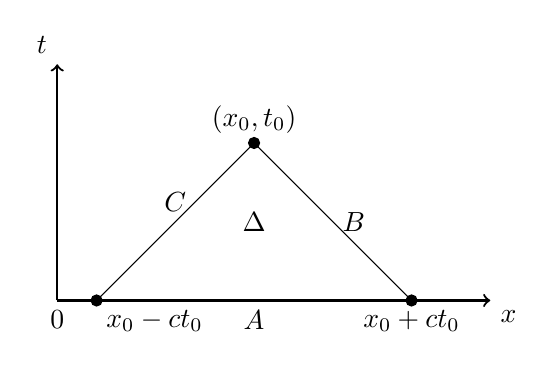
\begin{tikzpicture}

\draw[thick,->] (0.5,0) -- (6,0) node[anchor=north west] {$x$};
\draw[thick,->] (0.5,0) -- (0.5,3) node[anchor=south east] {$t$};
\draw (0.5 cm, 0pt) node[anchor=north] {$0$};

\draw (1,0) -- (3,2);
\draw (5,0) -- (3,2);
\filldraw[black] (3,2) circle (2pt) node[anchor=south] {$(x_0, t_0)$};
\filldraw[black] (1,0) circle (2pt) node[anchor=north west] {$x_0 - ct_0$};
\filldraw[black] (5,0) circle (2pt) node[anchor=north] {$x_0 + ct_0$};

\node[] at (3, 1) {$\Delta$};
\node[anchor=north] at (3, 0) {$A$};
\node[anchor=west] at (4, 1) {$B$};
\node[anchor=south] at (2, 1) {$C$};
\end{tikzpicture}
\end{center}

Từ tam giác trên, ta lấy tích phân hai vế phương trình truyền sóng như sau:

\begin{equation*}
    \iint_{\Delta} F(x, t)dxdt = \iint_{\Delta} (u_{tt} - c^2u_{xx})dxdt
\end{equation*}

Áp dụng công thức Green, ta thu được:
\begin{equation*}
    \iint_{\Delta} F(x, t)dxdt = \oint_{\partial \Delta} (-c^2u_x dt - u_t dx)
\end{equation*}

Biên $\partial \Delta$ thực chất là hợp của ba đoạn thằng $A$, $B$ và $C$ (như trên hình vẽ), vì vậy có thể tách công thức tích phân trên biên thành ba phần nhỏ như sau:

\begin{equation*}
\oint_{\partial \Delta} (-c^2u_x dt - u_t dx) = \int_A (-c^2u_x dt - u_t dx) + \int_B (-c^2u_x dt - u_t dx) + \int_C (-c^2u_x dt - u_t dx)
\end{equation*}

Tại cạnh đáy $A$, vì $t$ luôn bằng $0$, từ điều kiện ban đầu, dễ thấy:

\begin{equation*}
\int_A (-c^2u_x dt - u_t dx) = -\int_{x_0 - ct_0}^{x_0 + ct_0} u_t(x, 0)\, dx = -\int_{x_0 - ct_0}^{x_0 + ct_0} g(x) \,dx
\end{equation*}

Ở cạnh $B$, có $x + ct = x_0 + ct_0$, từ đây $dx = -cdt$, nên:
\begin{equation*}
    \int_B (-c^2u_x dt - u_t dx) = c\int_B (c^2u_x dt + u_t dx) = c[u(x_0,t_0) - u(x_0 + ct_0, 0)] = c[u(x_0,t_0) - f(x_0 + ct_0)]
\end{equation*}

Tính toán tương tự với $C$, ta cũng sẽ thu được:
\begin{equation*}
    \int_C (-c^2u_x dt - u_t dx) = -c[f(x_0 - ct_0) - u(x_0,t_0)]
\end{equation*}

Tính tổng của tích phân đường ba cạnh trên, ta thu được kết quả cuối cùng:

\begin{equation*}
\oint_{\partial \Delta} (-c^2u_x dt - u_t dx) = c[2u(x_0, t_0) - f(x_0 - ct_0) - f(x_0 + ct_0)] -\int_{x_0 - ct_0}^{x_0 + ct_0} g(x) \,dx
\end{equation*}

Rút $u(x_0, t_0)$ ra ngoài, ta thu được:

\begin{equation*}
u(x_0, t_0) = \frac{f(x_0 + ct_0) + f(x_0 - ct_0)}{2} + \frac{1}{2c}\int_{x_0 - ct_0}^{x_0 + ct_0} g(x)dx + \frac{1}{2c} \iint_{\Delta} F(x,t)dx dt
\end{equation*}

Giờ với mọi điểm $(x, t)$ bất kì, ta có công thức nghiệm tổng quát:

\begin{equation*}
u(x, t) = \frac{f(x + ct) + f(x - ct)}{2} + \frac{1}{2c}\int_{x - ct}^{x + ct} g(x)dx + \frac{1}{2c} \iint_{\Delta} F(\zeta,\tau)d\zeta d\tau
\end{equation*}

Công thức này cũng được gọi là \emph{công thức d'Alembert}

Khá thú vị rằng khi ta thay đúng $F(x, y)$ = 0, ta cũng sẽ thu được công thức d'Alembert của phương trình truyền sóng thuần nhất.

\section{Tài liệu tham khảo}
\begin{itemize}
    \item Các bài viết liên quan đến phương trình truyền sóng 1D --- TS. Đặng Anh Tuấn ---  \href{https://bomongiaitich.wordpress.com}{Blog Giải tích}
    \item ``An Introduction to Partial Differential Equation'' --- Y. Pinchover, J. Rubinstein --- ISBN 1-502-60323-X
    \item ``Partial differential equation'' --- Dr. C. Tisdel --- \href{https://www.youtube.com/playlist?list=PLGCj8f6sgswntUil8yzohR_qazOfYZCg_}{Playlist}
    \item ``Wave Equation'' --- PhD. G. Strang --- MIT OpenCourseWare --- \href{https://youtu.be/9TQCKWWAVjM}{Video}
    \item ``Math 124A/215A, Lecture 17'' --- PhD. V. Grigoryan --- Đại học Santa Barbara, California --- \href{http://web.math.ucsb.edu/~grigoryan/124A/lecs/lec17.pdf}{Lecture 17}
\end{itemize}
\end{document}
